% Options for packages loaded elsewhere
\PassOptionsToPackage{unicode}{hyperref}
\PassOptionsToPackage{hyphens}{url}
%
\documentclass[
  man]{apa7}
\usepackage{amsmath,amssymb}
\usepackage{iftex}
\ifPDFTeX
  \usepackage[T1]{fontenc}
  \usepackage[utf8]{inputenc}
  \usepackage{textcomp} % provide euro and other symbols
\else % if luatex or xetex
  \usepackage{unicode-math} % this also loads fontspec
  \defaultfontfeatures{Scale=MatchLowercase}
  \defaultfontfeatures[\rmfamily]{Ligatures=TeX,Scale=1}
\fi
\usepackage{lmodern}
\ifPDFTeX\else
  % xetex/luatex font selection
\fi
% Use upquote if available, for straight quotes in verbatim environments
\IfFileExists{upquote.sty}{\usepackage{upquote}}{}
\IfFileExists{microtype.sty}{% use microtype if available
  \usepackage[]{microtype}
  \UseMicrotypeSet[protrusion]{basicmath} % disable protrusion for tt fonts
}{}
\makeatletter
\@ifundefined{KOMAClassName}{% if non-KOMA class
  \IfFileExists{parskip.sty}{%
    \usepackage{parskip}
  }{% else
    \setlength{\parindent}{0pt}
    \setlength{\parskip}{6pt plus 2pt minus 1pt}}
}{% if KOMA class
  \KOMAoptions{parskip=half}}
\makeatother
\usepackage{xcolor}
\usepackage{graphicx}
\makeatletter
\def\maxwidth{\ifdim\Gin@nat@width>\linewidth\linewidth\else\Gin@nat@width\fi}
\def\maxheight{\ifdim\Gin@nat@height>\textheight\textheight\else\Gin@nat@height\fi}
\makeatother
% Scale images if necessary, so that they will not overflow the page
% margins by default, and it is still possible to overwrite the defaults
% using explicit options in \includegraphics[width, height, ...]{}
\setkeys{Gin}{width=\maxwidth,height=\maxheight,keepaspectratio}
% Set default figure placement to htbp
\makeatletter
\def\fps@figure{htbp}
\makeatother
\setlength{\emergencystretch}{3em} % prevent overfull lines
\providecommand{\tightlist}{%
  \setlength{\itemsep}{0pt}\setlength{\parskip}{0pt}}
\setcounter{secnumdepth}{-\maxdimen} % remove section numbering
% Make \paragraph and \subparagraph free-standing
\ifx\paragraph\undefined\else
  \let\oldparagraph\paragraph
  \renewcommand{\paragraph}[1]{\oldparagraph{#1}\mbox{}}
\fi
\ifx\subparagraph\undefined\else
  \let\oldsubparagraph\subparagraph
  \renewcommand{\subparagraph}[1]{\oldsubparagraph{#1}\mbox{}}
\fi
\newlength{\cslhangindent}
\setlength{\cslhangindent}{1.5em}
\newlength{\csllabelwidth}
\setlength{\csllabelwidth}{3em}
\newlength{\cslentryspacingunit} % times entry-spacing
\setlength{\cslentryspacingunit}{\parskip}
\newenvironment{CSLReferences}[2] % #1 hanging-ident, #2 entry spacing
 {% don't indent paragraphs
  \setlength{\parindent}{0pt}
  % turn on hanging indent if param 1 is 1
  \ifodd #1
  \let\oldpar\par
  \def\par{\hangindent=\cslhangindent\oldpar}
  \fi
  % set entry spacing
  \setlength{\parskip}{#2\cslentryspacingunit}
 }%
 {}
\usepackage{calc}
\newcommand{\CSLBlock}[1]{#1\hfill\break}
\newcommand{\CSLLeftMargin}[1]{\parbox[t]{\csllabelwidth}{#1}}
\newcommand{\CSLRightInline}[1]{\parbox[t]{\linewidth - \csllabelwidth}{#1}\break}
\newcommand{\CSLIndent}[1]{\hspace{\cslhangindent}#1}
\ifLuaTeX
\usepackage[bidi=basic]{babel}
\else
\usepackage[bidi=default]{babel}
\fi
\babelprovide[main,import]{english}
% get rid of language-specific shorthands (see #6817):
\let\LanguageShortHands\languageshorthands
\def\languageshorthands#1{}
% Manuscript styling
\usepackage{upgreek}
\captionsetup{font=singlespacing,justification=justified}

% Table formatting
\usepackage{longtable}
\usepackage{lscape}
% \usepackage[counterclockwise]{rotating}   % Landscape page setup for large tables
\usepackage{multirow}		% Table styling
\usepackage{tabularx}		% Control Column width
\usepackage[flushleft]{threeparttable}	% Allows for three part tables with a specified notes section
\usepackage{threeparttablex}            % Lets threeparttable work with longtable

% Create new environments so endfloat can handle them
% \newenvironment{ltable}
%   {\begin{landscape}\centering\begin{threeparttable}}
%   {\end{threeparttable}\end{landscape}}
\newenvironment{lltable}{\begin{landscape}\centering\begin{ThreePartTable}}{\end{ThreePartTable}\end{landscape}}

% Enables adjusting longtable caption width to table width
% Solution found at http://golatex.de/longtable-mit-caption-so-breit-wie-die-tabelle-t15767.html
\makeatletter
\newcommand\LastLTentrywidth{1em}
\newlength\longtablewidth
\setlength{\longtablewidth}{1in}
\newcommand{\getlongtablewidth}{\begingroup \ifcsname LT@\roman{LT@tables}\endcsname \global\longtablewidth=0pt \renewcommand{\LT@entry}[2]{\global\advance\longtablewidth by ##2\relax\gdef\LastLTentrywidth{##2}}\@nameuse{LT@\roman{LT@tables}} \fi \endgroup}

% \setlength{\parindent}{0.5in}
% \setlength{\parskip}{0pt plus 0pt minus 0pt}

% Overwrite redefinition of paragraph and subparagraph by the default LaTeX template
% See https://github.com/crsh/papaja/issues/292
\makeatletter
\renewcommand{\paragraph}{\@startsection{paragraph}{4}{\parindent}%
  {0\baselineskip \@plus 0.2ex \@minus 0.2ex}%
  {-1em}%
  {\normalfont\normalsize\bfseries\itshape\typesectitle}}

\renewcommand{\subparagraph}[1]{\@startsection{subparagraph}{5}{1em}%
  {0\baselineskip \@plus 0.2ex \@minus 0.2ex}%
  {-\z@\relax}%
  {\normalfont\normalsize\itshape\hspace{\parindent}{#1}\textit{\addperi}}{\relax}}
\makeatother

% \usepackage{etoolbox}
\makeatletter
\patchcmd{\HyOrg@maketitle}
  {\section{\normalfont\normalsize\abstractname}}
  {\section*{\normalfont\normalsize\abstractname}}
  {}{\typeout{Failed to patch abstract.}}
\patchcmd{\HyOrg@maketitle}
  {\section{\protect\normalfont{\@title}}}
  {\section*{\protect\normalfont{\@title}}}
  {}{\typeout{Failed to patch title.}}
\makeatother

\usepackage{xpatch}
\makeatletter
\xapptocmd\appendix
  {\xapptocmd\section
    {\addcontentsline{toc}{section}{\appendixname\ifoneappendix\else~\theappendix\fi\\: #1}}
    {}{\InnerPatchFailed}%
  }
{}{\PatchFailed}
\keywords{keyword, more keyword, crazy keyword\newline\indent Word count: X}
\DeclareDelayedFloatFlavor{ThreePartTable}{table}
\DeclareDelayedFloatFlavor{lltable}{table}
\DeclareDelayedFloatFlavor*{longtable}{table}
\makeatletter
\renewcommand{\efloat@iwrite}[1]{\immediate\expandafter\protected@write\csname efloat@post#1\endcsname{}}
\makeatother
\usepackage{csquotes}
\makeatletter
\renewcommand{\paragraph}{\@startsection{paragraph}{4}{\parindent}%
  {0\baselineskip \@plus 0.2ex \@minus 0.2ex}%
  {-1em}%
  {\normalfont\normalsize\bfseries\typesectitle}}

\renewcommand{\subparagraph}[1]{\@startsection{subparagraph}{5}{1em}%
  {0\baselineskip \@plus 0.2ex \@minus 0.2ex}%
  {-\z@\relax}%
  {\normalfont\normalsize\bfseries\itshape\hspace{\parindent}{#1}\textit{\addperi}}{\relax}}
\makeatother

\raggedbottom

\usepackage{hhline}

\setlength{\parskip}{0pt}

\ifLuaTeX
  \usepackage{selnolig}  % disable illegal ligatures
\fi
\IfFileExists{bookmark.sty}{\usepackage{bookmark}}{\usepackage{hyperref}}
\IfFileExists{xurl.sty}{\usepackage{xurl}}{} % add URL line breaks if available
\urlstyle{same}
\hypersetup{
  pdftitle={Automatically Extracting ERP Component Latencies Using a Template Matching Algorithm},
  pdfauthor={Sven Lesche1},
  pdflang={en-EN},
  pdfkeywords={keyword, more keyword, crazy keyword},
  hidelinks,
  pdfcreator={LaTeX via pandoc}}

\title{Automatically Extracting ERP Component Latencies Using a Template Matching Algorithm}
\author{Sven Lesche\textsuperscript{1}}
\date{}


\shorttitle{Template Matching}

\authornote{

Author Notes go here.

The authors made the following contributions. Sven Lesche: Conceptualization, Writing - Original Draft Preparation, Writing - Review \& Editing.

Correspondence concerning this article should be addressed to Sven Lesche, Im Neuenheimer Feld 695, 69120 Heidelberg. E-mail: \href{mailto:sven.lesche@psychologie.uni-heidelberg.de}{\nolinkurl{sven.lesche@psychologie.uni-heidelberg.de}}

}

\affiliation{\vspace{0.5cm}\textsuperscript{1} Ruprecht-Karls-University Heidelberg}

\abstract{%
One or two sentences providing a \textbf{basic introduction} to the field, comprehensible to a scientist in any discipline.

Two to three sentences of \textbf{more detailed background}, comprehensible to scientists in related disciplines.

One sentence clearly stating the \textbf{general problem} being addressed by this particular study.

One sentence summarizing the main result (with the words ``\textbf{here we show}'' or their equivalent).

Two or three sentences explaining what the \textbf{main result} reveals in direct comparison to what was thought to be the case previously, or how the main result adds to previous knowledge.

One or two sentences to put the results into a more \textbf{general context}.

Two or three sentences to provide a \textbf{broader perspective}, readily comprehensible to a scientist in any discipline.
}



\begin{document}
\maketitle

\hypertarget{history-of-extraction-methods}{%
\section{History of Extraction Methods}\label{history-of-extraction-methods}}

In cognitive neuroscience, the accurate extraction of latencies of event-related potentials (ERPs) stands as a crucial step in understanding the timing of neural processes that underlie cognitive functions (\protect\hyperlink{ref-luck2014introduction}{Luck, 2014}). In studies focusing on individual differences an objective, efficient, valid and reliable extraction process is paramount. Algorithms allow efficient and objective approaches to latency extraction, but often prove unreliable and invalid due to ERPs with low signal-to-noise ratios (\protect\hyperlink{ref-kiesel2008measurement}{Kiesel et al., 2008}; \protect\hyperlink{ref-sadus2023multiverse}{Sadus et al., 2023}; \protect\hyperlink{ref-schubert2023robust}{Schubert et al., 2023}; \protect\hyperlink{ref-clayson2023noise}{\textbf{clayson2023noise?}}). To deal with this issue, researchers often forgo algorithms and manually inspect each ERP, identifying patterns reflecting the component of interest by hand (\protect\hyperlink{ref-sadus2023multiverse}{Sadus et al., 2023}). Manual extraction is a labor-intensive and time-consuming endeavor, improving reliability and validity at the cost of objectivity and efficiency. This paper introduces a novel algorithm for the automatic extraction of ERP latencies using template matching. We aim to show that our algorithm improves on existing approaches and enables more efficient, objective, reliable and valid extraction of ERP latencies.

\hypertarget{peak-latency-algorithms}{%
\subsection{Peak Latency Algorithms}\label{peak-latency-algorithms}}

Automatically extracting component latencies has long been a goal in ERP research. \emph{Peak latency} algorithms present the earliest attempt at automating the latency extraction process. The peak latency approach involves finding the point in time within a set measurement window that displays the largest voltage deflection in the appropriate direction. This approach remains the most commonly used way of latency extraction to-date (\protect\hyperlink{ref-kiesel2008measurement}{Kiesel et al., 2008}; \protect\hyperlink{ref-liesefeld2018estimating}{Liesefeld, 2018}), partially due to the ease of its implementation and low computational requirements (\protect\hyperlink{ref-donchin1978multivariate}{Donchin \& Heffley, 1978}). However, ease of implementation is accompanied by several drawbacks.

Firstly, peak latency approaches are blind to the general structure within the ERP signal. They locate the point in time with the largest voltage deflection within the measurement window. The ``true'' maximum signal may lay just outside of the measurement window, resulting in the algorithm picking an outside edge of the window, even though the signal increases in amplitude just following that time-point. The simple \emph{peak latency} algorithm can be extended to only consider maxima inside the measurement window which are also larger than the surrounding data-points (\protect\hyperlink{ref-luck2014introduction}{Luck, 2014}). A spike just on the edge of the measurement window will not meet these criteria. This approach protects against the influence of noise or surrounding components on the edges of the measurement window, but remains vulnerable to high frequency noise inducing peaks inside the measurement window.

Due to high frequency noise, the maximum voltage deflection may not reflect the true point in time at which the process underlying the component reaches its maximum. Rather it may be the result of high frequency noise inducing a spike in the signal, independent of any cognitive process. This is problematic especially in later ERP components, as the broader measurement window most commonly applied increases the likelihood of high frequency noise inducing the maximum voltage deflection (\protect\hyperlink{ref-clayson2013noise}{Clayson et al., 2013}).

The sensitivity of the peak latency approach to the size of the measurement window is further increased by the \emph{superimposition problem} (\protect\hyperlink{ref-luck2014introduction}{Luck, 2014}). In larger measurement windows, later components can already influence the amplitude on the outer ranges of the measurement window. Researchers have to carefully choose the measurement window in order to include most of the signal related to the component of interest while simultaneously excluding influences of other components.

Lastly, as Luck (\protect\hyperlink{ref-luck2014introduction}{2014}) so aptly states: \emph{There is nothing special about the point at which the voltage reaches a local maximum}. The largest deflection does not inherently relate to any physiological or psychological process and may not even reflect the true maximum of the component of interest. Luck (\protect\hyperlink{ref-luck2005ten}{2005}) visually demonstrates how peak latency may be a result of the overlap of multiple components and not related to any single component.

\hypertarget{fractional-area-latency-algorithms}{%
\subsection{Fractional Area Latency Algorithms}\label{fractional-area-latency-algorithms}}

\emph{Fractional Area Latency} approaches hope to remedy some of the problems associated with peak latency algorithms. This technique revolves around the area under the ERP signal in a given measurement window. The goal is to find the point in time that divides that area under the signal into a given fraction to the left and right of it. The time-point halving the area under the signal, for example, is referred to as the \emph{50\% area latency}. This approach is much less susceptible to the influence of high frequency noise, as short spikes in the signal do not have a strong impact on the area under the signal (\protect\hyperlink{ref-liesefeld2018estimating}{Liesefeld, 2018}). Area latency approaches remain highly dependent on the measurement window (\protect\hyperlink{ref-luck2014introduction}{Luck, 2014}). Choosing a shorter window may result in only a part of the area of the component of interest being captured. A wider measurement window on the other hand might be influenced by surrounding components. \emph{Fractional Area} measures thus work best for investigating an isolated component (\protect\hyperlink{ref-luck2014introduction}{Luck, 2014}), limiting the applicability of area latency algorithms.

\hypertarget{jackknifing}{%
\subsection{Jackknifing}\label{jackknifing}}

Another approach towards dealing with noisy subject-level ERPs is to try and mitigate that noise by averaging multiple subject-level ERPs. This technique is referred to as \emph{jackknifing} (\protect\hyperlink{ref-miller1998jackknife}{Miller et al., 1998}). It uses the grand average of \(N\) subject-level ERPs and generates \(N\) sub-grand averages by removing one of the subject-level ERPs. This averaging procedure results in \(N\) ERPs with higher signal-to-noise ratios. Both \emph{peak} and \emph{area} based measures can then be applied to the jackknifed data to extract latencies. As any two jackknifed signals share \(\frac{N-2}{N} * 100\) percent of the subject-level signals that are averaged with each other, each jackknifed sub-average is quite similar to all others. This artificially decreases the error variance, which needs to be corrected for when testing for differences between groups (\protect\hyperlink{ref-ulrich2001using}{Ulrich \& Miller, 2001}). Because latencies extracted from jackknifed ERPs are based on averaged waveforms, they can not readily be associated with any single subject, preventing this method from generating individual-level latency estimates needed for individual differences research. This problem was addressed by (\protect\hyperlink{ref-smulders2010simplifying}{Smulders, 2010}) who introduced a transformation able to generate individual-level latency estimates.

\hypertarget{comparison-of-algorithms}{%
\subsection{Comparison of Algorithms}\label{comparison-of-algorithms}}

Kiesel et al. (\protect\hyperlink{ref-kiesel2008measurement}{2008}) applied these different algorithms, as well as a few additional approaches not mentioned here, to a variety of ERP components. They simulated latency differences of the visual and auditory N1, the N2pc and the P3 and frequency-related P3 and tested single-participant approaches and jackknife-approaches combined with peak latency, fractional area latency, relative criteria and baseline deviation methods on their ability to detect these effects. The most widely used technique of single-participant approaches combined with peak latency extraction proved to not be the most best method to detect latency effects. Its effectiveness decreases even further as the signal-to-noise ratio decreases. Overall, jackknifing ERPs and using the relative criterion technique or the fractional area latency technique was shown to be the best approach across the components and datasets they analyzed.

Kiesel et al. (\protect\hyperlink{ref-kiesel2008measurement}{2008}) were concerned with extracting condition differences in ERP research. While this is important, techniques applied in individual differences research have to extract latencies from subject-level ERPs and produce both reliable and valid estimates. Kiesel et al. (\protect\hyperlink{ref-kiesel2008measurement}{2008}) did not assess psychometric properties of latency estimates. Addressing this gap in research, Sadus et al. (\protect\hyperlink{ref-sadus2023multiverse}{2023}) investigated the influence of different preprocessing strategies and latency extraction techniques on psychometric properties of the latency values generated as well as the ability to detect an age-related effect in P3 latency. They varied the strength of the low-pass filter applied to the data, used both single-participant and jackknife approaches and extracted latencies either automatically or manually, using either a peak latency or area latency approach. Both the size of the effect and the psychometric properties, such as reliability or homogeneity of the latency values, varied between the different analysis strategies. No combination of preprocessing steps and extraction method proved best across all tasks and groups. Only 7 out of 40 possible pipelines generated consistently desirable reliabilities (\(r_{tt} \ge .70\)), homogeneities (\(r_{h} \ge .50\)) and effect sizes (\(.03 \le \omega^2 <.80\)). All of those seven pipelines used manual extraction methods either based on peak or area latencies. While automated extraction methods would improve both efficiency and objectivity, fully automated approaches failed to generate consistently reliable and valid latency measures (\protect\hyperlink{ref-sadus2023multiverse}{Sadus et al., 2023}; \protect\hyperlink{ref-schubert2023robust}{Schubert et al., 2023}). Yet, manual extraction methods are highly time-consuming and impede reproducibility. We hope to show that our algorithm can match the performance of manual extraction while providing a more efficient and objective approach for extracting individual component latency values.

\hypertarget{template-matching}{%
\section{Template Matching}\label{template-matching}}

The shortcomings of prior algorithms may be due to none of them aiming to replicate human behavior and rather focusing on generating similar decisions, not similar decision processes. Our proposed algorithm more closely resembles the process expert ERP researches employ.

\hypertarget{template-matching-1}{%
\subsection{template matching}\label{template-matching-1}}

\hypertarget{introduction}{%
\subsubsection{Introduction}\label{introduction}}

During latency extraction, most researchers have some mental representation of what the component \emph{should} look like and where it \emph{should} generally appear. When visually inspecting ERP signals, their goal is to identify a pattern within the signal that resembles the component of interest in shape, size and location.

Finding a given pattern inside a noisy signal is not a novel task. Algorithms aiming to detect the appearance of a pattern, a \emph{template}, inside audio-, video- or radio signals have been around for over 50 years, and a large amount of research has gone into optimizing these \emph{template matching} algorithms (\protect\hyperlink{ref-briechle2001template}{Briechle \& Hanebeck, 2001}; \protect\hyperlink{ref-brunelli2009template}{Brunelli, 2009}; \protect\hyperlink{ref-lewis1995fast}{Lewis, 1995}; \protect\hyperlink{ref-mahalakshmi2012image}{Mahalakshmi et al., 2012}).

No matter the implementation details of a particular template matching algorithm, all aim to answer the question ``Does this (smaller) template appear in my (larger) signal?''. To achieve this, a researcher needs to specify two things. First, the template they want to search the signal for. And second, the \emph{similarity measure} which quantifies how well the template fits in a given spot of the signal.

\hypertarget{similarity-measures}{%
\subsubsection{Similarity measures}\label{similarity-measures}}

Specifying the template is mostly a philosophical question dependent on the specific task and type of signal. Choosing a similarity measure on the other hand is much more methodological. Across a number of papers, several different similarity measures have been proposed. They follow one of two general lines of thought (\protect\hyperlink{ref-brunelli1997template}{Brunelli \& Poggiot, 1997}; \protect\hyperlink{ref-goshtasby1984two}{Goshtasby et al., 1984}). The first type of similarity measure aims to minimize some value reflecting the distance between template and the signal. The second type aims to maximize some form of correlation between signal and template. We have chosen to implement algorithms based on two of the possible measures, one minimizing the Sum of Squared Differences and one maximizing the correlation between the template and the signal. We wanted to implement both a similarity measure following a traditional distance-minimization approach and a correlational approach in order to gauge the efficacy of these approaches when applied to our field of research. We call the algorithm based on minimization of the squared difference \emph{MINSQ} and the algorithm based on maximization of the correlation \emph{CORR}.

\hypertarget{template-generation}{%
\subsubsection{Template generation}\label{template-generation}}

Finding an appropriate template is sometimes more challenging. Depending on the field, the template to search for is easily specified. If you are looking to extract a particular audio-signal from a recording or some specific object in an image you can easily use that object as a template. The difficulty increases if it is not exactly certain what template you are looking for. Recent research in image processing has attempted to use template matching to process faces (\protect\hyperlink{ref-brunelli2009template}{Brunelli, 2009}). You cannot just use ``the ideal set of eyes'' to identify a face. Each person comes with their own set of eyes, different from all others in some quantifiable way. A similar issue accompanies attempts of template matching approaches in ERP research. The variance in ERP signals introduced by the task or the sample of participants hinders a successful implementation of template matching algorithms using only one idealized template over all types of studies. Finding a template that reflects the influence of the task or the sample, equivalent to finding the person who's eyes you are looking for, will significantly improve performance.

\hypertarget{prior-attempts}{%
\subsection{Prior attempts}\label{prior-attempts}}

There have been some attempts at using an idealized signal structure as a template to identify ocular artifacts in noisy subject-level data (\protect\hyperlink{ref-li2006automatic}{Li et al., 2006}) or to predict subject behavior on a single trial level (\protect\hyperlink{ref-william2020erp}{William et al., 2020}). These studies were able to successfully implement template matching algorithms. However, they were not concerned with estimating the timing of components, but only interested in detection of a specific signal.

Borst and Anderson (\protect\hyperlink{ref-borst2015discovery}{2015}) and Anderson et al. (\protect\hyperlink{ref-anderson2016discovery}{2016}) developed a machine-learning approach that aims to discover cognitive processing stages on a single trial level. In a first step, their algorithm makes use of multivariate pattern analysis to detect ``bumps'' in the EEG signal representing the onset of a new cognitive state. They assumed that entry into a new state would be accompanied by a bump in all electrodes similar to a 50 ms half-sine. This 50 ms half-sine then serves as a template with which their algorithm tries to detect those ``bumps'' in activity. However, their assumptions regarding the template and the location of activity are somewhat crude generalizations made necessary by noisy single trial data. Using template matching to extract component latencies from ERPs requires a more informative template.

\hypertarget{our-solution}{%
\subsection{our solution}\label{our-solution}}

A simple approach towards designing a more informative template would be to generate an idealized component structure. Prior knowledge about the shape, size and location about the component of interest could then be made use of. One could draw up ``the perfect P3'' and attempt to use this as a template. This would neglect the experiment-specific and task-specific variance in the morphology of ERP components, resulting in a template that does not optimally reflect the data. We addressed this problem by using the grand average as an experiment-specific template of the component of interest that will reflect influences of the task and sample on the morphology of the idealized ERP component. We use the grand average and the specific window in which the component of interest occurs as a template to match to subject-level ERPs. The grand average lends itself as a template because it has a higher signal-to-noise ratio than any individual subject-level ERP while still being influenced by experiment-specific changes in component morphology. It is by definition the mean of all subject-level ERPs and thus minimizes the sum of squared deviations between each subject-level ERP and itself. Thus, across all subjects, it is the best approximation for each subject-level ERP. Researchers can (and already often do) use the grand average to gather insight into the time window in which the component of interest occurs (\protect\hyperlink{ref-kiesel2008measurement}{Kiesel et al., 2008}).

\hypertarget{differences-to-other-template-matching-studies}{%
\subsubsection{Differences to other template matching studies}\label{differences-to-other-template-matching-studies}}

The goal of our algorithm is to quantify individual differences in the latency of ERP components, not only the presence of a particular ERP component. This is similar to facial recognition not only detecting the presence of eyes, but also determining the person the eyes belong to. We do not only aim to detect the presence of a component, but also aim to measure individual differences in shape, size and location of the component.

To achieve this, we introduce variability into the template reflecting individual differences in the morphology of the component. This transformation generates versions of the grand average as a template with different amplitudes and locations of the component of interest. Crudely, each transformation reflects the idealized component if it had higher vs.~lower overall amplitudes and earlier vs.~later latencies of the component of interest. We can simulate how the template would look like if the component had any given latency. Determining which transformation of the template best fits a given subject-level ERP will allow us to investigate individual differences.

\hypertarget{subject-level-transformations-as-the-goal}{%
\subsection{Subject-level transformations as the goal}\label{subject-level-transformations-as-the-goal}}

We introduce variability in the template through two sources, amplitude and latency. Variability in amplitude is controlled by the parameter \(a\), variability in latency by the parameter \(b\). Amplitude of the template is varied by multiplying the whole template-signal by parameter \(a\). Latency is varied by ``stretching'' or ``squishing'' the template along the x-axis (see Figure \ref{fig:b-scale-example}). The parameter \(b\) controls the strength of this transformation. Possible transformations of the template are then compared to the signal and their similarity is evaluated. Recovering the transformation parameters \([a, b]\) that lead to the best match between template and signal thus allows us to describe individual differences in the latency of a component. To recover latencies of the component of interest from the optimal transformation parameter, researchers need to specify a time-point of the grand average denoting the latency of the component of interest. The optimal transformation parameters are then applied to the grand average latency to recover the subject-level latency of the component.



\begin{figure}
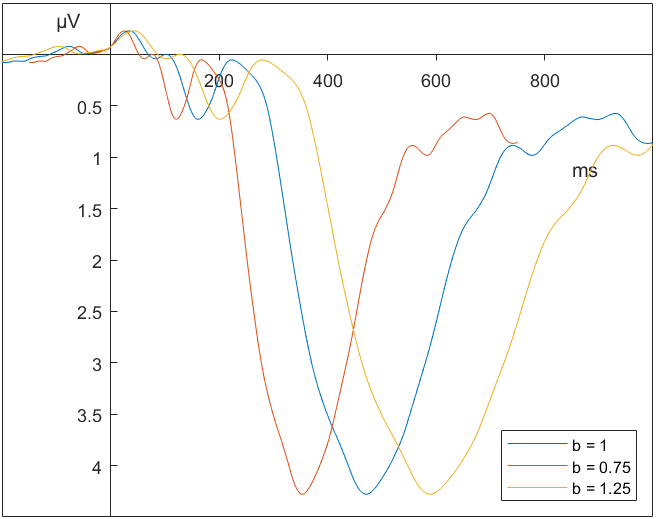
\includegraphics[width=0.75\linewidth]{images/b_scale} \caption{Scaling Templates Horizontally}\label{fig:b-scale-example}
\end{figure}

\hypertarget{why-our-algorithm-may-perform-better}{%
\subsection{Why our algorithm may perform better}\label{why-our-algorithm-may-perform-better}}

This algorithm aims to address some of the issues faced by other algorithms. It makes use of the entire component structure to construct the template that is matched to subject-level ERPs. This reflects the decision process of expert ERP researchers and enables an intuitive understanding of the decisions made by our algorithm. Because the similarity measures take the whole component structure into account, they are robust to peaks introduced by high frequency noise. Furthermore, the measurement window set by the researcher only impacts the size and shape of the template. It has no direct connection to the subject-level ERP. The influence of measurement windows on the latencies extracted should thus be lower than in peak latency or area latency algorithms. Lastly, it is important to note that this is not a machine learning algorithm with a neural net representing some ``black box'' decision making algorithm. Simplicity and traceability of the decision process was an express goal, allowing more insight into the benefits and drawbacks of our algorithm.

\hypertarget{the-present-study}{%
\subsection{The present study}\label{the-present-study}}

In order to compare the quality of our proposed algorithm we will reanalyze the same data analyzed by Sadus et al. (\protect\hyperlink{ref-sadus2023multiverse}{2023}). We compare the psychometric properties of our algorithm to those of previously established algorithms, investigate the impact of different preprocessing steps and evaluate the correlation between latencies extracted by our algorithm and those extracted manually by an expert ERP researcher.

In their study, Sadus et al. (\protect\hyperlink{ref-sadus2023multiverse}{2023}) extracted latencies of the P3b component, henceforth simply referred to as P3. The P3 is a centro-parietal positive-going component, peaking around 300 ms after stimulus onset. It is a late higher-order cognitive component associated with higher-order cognitive processes (\protect\hyperlink{ref-donchin1981surprise}{Donchin, 1981}; \protect\hyperlink{ref-duncan1981young}{Duncan-Johnson, 1981}; \protect\hyperlink{ref-mccarthy1981metric}{McCarthy \& Donchin, 1981}; \protect\hyperlink{ref-polich2007updating}{Polich, 2007}, \protect\hyperlink{ref-polich2012neuropsychology}{2012}; \protect\hyperlink{ref-verleger2020effects}{Verleger, 2020}). A number of studies have demonstrated a large effect of age on the latency of the P3 across a number of tasks with older participants displaying systematically later P3 peaks than their younger counterparts (\protect\hyperlink{ref-friedman2012components}{Friedman, 2011}; \protect\hyperlink{ref-scrivano2022behavioral}{Scrivano \& Kieffaber, 2022}). In a multiverse approach Sadus et al. (\protect\hyperlink{ref-sadus2023multiverse}{2023}) tested several extraction methods with varying preprocessing steps in their ability to detect this age effect. They used three tasks, each measuring one of the executive functions proposed by Miyake et al. (\protect\hyperlink{ref-miyake2000unity}{2000}). To measure the functions \emph{updating}, \emph{shifting} and \emph{inhibition}, they employed an Nback, a Switching and a Flanker Task, respectively. Studying three different tasks allows us to gain insight into a larger variety of higher-order cognitive processing, improving the generalizability of our findings.

Nonetheless, we will restrict our analysis to extracting P3 latencies. The P3 usually has a broad and isolated structure with comparatively low influence of surrounding components {[}REF - kathrin?{]}. This makes the P3 one of the easier components for automated latency extraction approaches. After we can demonstrate proof-of-concept for P3 latency extraction, we will evaluate the algorithms ability to be extended to other ERP components.

We hope to show that a template matching approach using the grand average as a variable template can successfully extract P3 component latencies. Ideally, use of this algorithm will improve psychometric properties in comparison to prior algorithms, show high correlations with manually extracted data and present an objective and efficient way to extract ERP latencies.

\hypertarget{algorithm}{%
\section{Algorithm}\label{algorithm}}

\hypertarget{implementation-in-matlab-with-details}{%
\subsection{Implementation in Matlab with details}\label{implementation-in-matlab-with-details}}

We implemented the algorithm in MATLAB (Version 2022b) (\protect\hyperlink{ref-matlab2022b}{The Math Works, 2022}). The researcher specifies the name and polarity of the component of interest as well as the measurement window. This window is used to extract the template. In order to transform the template, we use MATLABs Curve Fitting Toolbox (\protect\hyperlink{ref-matlab2022b}{The Math Works, 2022}) to generate \emph{sum of sines} functions that fit to the data with \(R^2 \ge 0.999\). We then add an amplitude parameter \(a\) to the overall function in order to allow for scaling of the amplitude of the template and a frequency parameter \(b\) to all frequency terms in the sum of sines function to allow for ``squishing'' or ``stretching'' the template along the x-Axis. The resulting variable template is described by a function \(f(x, a, b)\) with \(n\) sine terms and their respective amplitude \(A_i\), frequency \(f_i\) and phase \(\phi_i\).

\[f(x, a, b) = \sum_{i = 1}^{n} a\cdot(A_isin(bf_ix + \phi_i)\]
As these transformations also change the measurement window, we chose to use the subject-level ERP as a template and keep the grand average untransformed as a signal. This reverse matching approach is only an implementation detail and does not affect any decisions made by the algorithm.

Depending on the similarity measure employed, we use different functions to find the set of optimal parameters \([a_j, b_j]\) that lead to the optimal transformation for a given subject \(j\).

\hypertarget{minsq}{%
\subsubsection{MINSQ}\label{minsq}}

The MINSQ algorithm minimizes the weighted sum \(S\) of squared differences \(d\) between the transformed subject signal and the grand average.
\[S = \sum_{i = 1}^{n}\omega_{i}d_{i}^2\]
This weighting vector \(\omega\) is computed as follows
\[\omega_i = 1+\mathbb{1}_{[t_{start}, t_{end}]}(x_i)(10 \cdot |\frac{y_i}{y_{max}}|)^2\]
Where
\[\mathbb{1}_{[t_{start}, t_{end}]}(x_i) = \begin{cases} 1 & \text{if $t_{start} \le x_i \le t_{end}$} \\ 0 & \text{otherwise}\end{cases}\]\([t_{start}, t_{end}]\) denotes the measurement window, \(y_{i}\) the signal strength of the \(i\)th element, \(y_{max}\) the maximum voltage deflection inside the measurement window and \(x_i\) the time of the \(i\)th element.

This places more emphasis on fitting the template within the measurement window specified and to places in the signal where the voltage deflection is high.

We use MATLABs \emph{fit} function to find optimal parameters \([a_j, b_j]\) with upper and lower bounds such that \(a_j \in [0, 50]; b_j \in [0.5, 3]\). As this function may be prone to converging on local minima, we initialize 5 different start points. The solution with the best correlation between transformed template and signal that multiple start points converged on is selected.

In cases where the subject-level ERP only has signal with deflections opposite of the deflection of the component of interest, it may occur that the parameter \(a_j \le 0\). In these cases, we attempt to re-match the signal with an added parameter \(d\) shifting the entire template up or down.
\[f(x, a,b, d) = d +\sum_{i = 1}^{n} a*(A_isin(b*f_ix + \phi_i)\]
Should the algorithm again converge on a solution with \(a_j \le 0\), the latency value is set to NA.

\hypertarget{corr}{%
\subsubsection{CORR}\label{corr}}

The CORR algorithm optimizes the parameters to produce the maximum correlation \(r_{st}\) between the transformed subject-level signal \(s\) and the grand average \(t\) for values in the measurement window.
\[r_{st} = \frac{\sum(s_i - \bar{s})(t_{i} - \bar{t})}{\sqrt{\sum(s_i - \bar{s})^2(t_{i} - \bar{t})^2}}\]
\(t\) represents the vector of values of the transformed subject ERP that are in the measurement window, \(s\) the vector of values of the grand average that are in the measurement window. As the correlation-coefficient is independent of translation and scaling, varying the parameter \(a_j\) will not impact the correlation \(r_{st}\). We therefore just set \(a_j = 1\) and only optimize \(b_j\).

We use MATLABs \emph{fminbnd} function to find the optimal transformation parameter \(b_j\) maximizing \(r_{st}\). This function will estimate the objective function for all values inside the given bounds \(b_j \in [0.5, 2]\) and converge on the global optimum. Hence, we do not need to initialize a number of different starting points here.

Both algorithms then return the transformation parameters \([a_j, b_j]\) that result in optimal similarity of transformed template and signal. We use the returned value of the parameter \(b_j\) to transform the component latency specified by the researcher in the grand average \(l_{GA}\) to the component latency of the subject-level ERP signal \(l_j\).
\[ l_j = l_{GA} * b_j \]

\hypertarget{review-methods}{%
\subsection{Review methods}\label{review-methods}}

Researchers can manually review all choices the algorithm has made in a custom-built user interface (see Figure \ref{fig:review-gui-example}). For both algorithms, we used the correlation between transformed template and signal as a fit-index. This can be used to only review those cases where the correlation between template and signal dips below a certain value, indicating low similarity between matched template and signal. We will investigate the additional benefits a manual review process provides over accepting the choices as-is or only automatically discarding those matches with correlations \(r_{st} \le .20\).



\begin{figure}
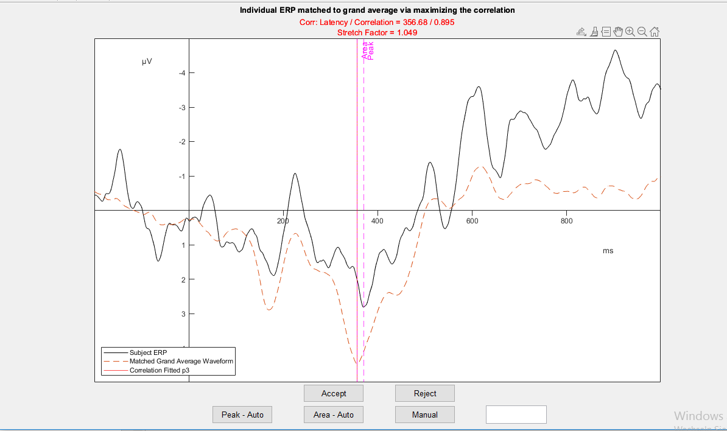
\includegraphics[width=0.75\linewidth]{images/review_gui_example} \caption{User Interface for Manual Review Process}\label{fig:review-gui-example}
\end{figure}

\hypertarget{data}{%
\section{Data}\label{data}}

The data used here were first published by Sadus et al. (\protect\hyperlink{ref-sadus2023multiverse}{2023}) and are a subset of the data collected by Löffler et al. (\protect\hyperlink{ref-loffler2022common}{2022}).

\hypertarget{participants}{%
\subsection{Participants}\label{participants}}

The data is comprised of 30 young participants (18-21 years old, mean age = 19.37, SD age = 0.76) and 30 old participants (50-60 years old, mean age = 55.83, SD age = 2.87). This sample was part of a larger study (\protect\hyperlink{ref-loffler2022common}{Löffler et al., 2022}) of which the 30 youngest and 30 oldest participants were selected. All participants had normal or corrected to normal vision. None of the participants had neurological or mental disorders, used psychotropic drugs, wore a pacemaker or suffered from red-green color vision deficiency. The participants provided informed consent prior to participation and received 75€ or course credit for participation. \textbf{ethics stuff?}

\hypertarget{tasks}{%
\subsection{Tasks}\label{tasks}}

Participants completed a set of 3 tasks: a Flanker Task, an Nback Task and a Switching Task. These tasks each measure one of the executive functions proposed by Miyake et al. (\protect\hyperlink{ref-miyake2000unity}{2000}). Löffler et al. (\protect\hyperlink{ref-loffler2022common}{2022}) programmed all tasks in MATLAB (\protect\hyperlink{ref-matlab2022b}{The Math Works, 2022}) using the software package Psychtoolbox (Version 3-0.13) (\protect\hyperlink{ref-brainard1997psychophysics}{Brainard \& Vision, 1997}; \protect\hyperlink{ref-kleiner2007psychtoolbox}{Kleiner et al., 2007}; \protect\hyperlink{ref-pelli1997videotoolbox}{Pelli \& Vision, 1997}). Stimuli were presented centrally on a black background. We instructed participants to respond as quickly and accurately as possible.

\hypertarget{flanker-task}{%
\subsubsection{Flanker Task}\label{flanker-task}}

We administered a standard Arrow Flanker task (\protect\hyperlink{ref-eriksen1974effects}{Eriksen \& Eriksen, 1974}) to measure participants' \emph{inhibition} ability. A central arrow pointing either to the left or to the right is flanked by two additional arrows to each side. These flanking arrows either point in the same or in the opposite direction as the central arrow. Participants have to respond by button press in which direction the central arrow pointed, disregarding the congruent or incongruent flanking arrows. Participants completed a set of practice trials and a total of 100 congruent and 100 incongruent trials.

\hypertarget{nback-task}{%
\subsubsection{Nback Task}\label{nback-task}}

We administered an adapted version of the Nback task from (\protect\hyperlink{ref-scharinger2015flanker}{Scharinger et al., 2015}) to measure participants' \emph{updating} abilities. A stream of letters is shown to the participant. In the 0-back condition, participants have to indicate by keypress whether the presented letter is equivalent to a target letter. In the 1-back condition, participants have to indicate whether the currently presented letter is the same as the letter presented one trial before or not. Löffler et al. (\protect\hyperlink{ref-loffler2022common}{2022}) also had participants complete a 2-back condition. We excluded this condition from our analysis as it did not produce clear ERPs. Participants completed a set of practice trials and a total of 96 trials per condition.

\hypertarget{switching-task}{%
\subsubsection{Switching Task}\label{switching-task}}

We administered a Switching task to measure participants' \emph{shifting} ability. A stream of colored digits ranging from 1 to 9 was presented. Participants had to indicate whether the digit was greater than or less than 5 or whether the digit was odd or even depending on the color of the stimulus. A colored fixation cross just prior to stimulus presentation cued the rule participants had to follow in the upcoming trial. Participants had to either follow the same rule as in the trial before or switch to the other rule. Participants completed a set of practice trials and 192 trials each in the repeat and in the switch condition.

\hypertarget{procedure}{%
\subsection{Procedure}\label{procedure}}

The original study consisted of three test sessions. The three tasks the present work focuses on were all administered in the first session. The second session also included EEG measurement with 3 additional tasks. The third session was used to measure intelligence and working memory capacity. No EEG measurements were taken here. In sessions including EEG measurements, participants were seated approximately 140cm away from a monitor in a sound-attenuated room.

\hypertarget{eeg-recording-and-processing}{%
\subsection{EEG recording and processing}\label{eeg-recording-and-processing}}

EEG was recorded using 32 equidistant Ag/AgCl scalp electrodes. Additional electrooculogram (EOG) measures were taken by two electrode placed above and below the left eye to correct for ocular artifacts. All impedances were kept below 5 kΩ. The signal was recorded with a sampling rate of 1000 Hz (band-pass 0.1 Hz - 100 Hz) and online-referenced to Cz. Following data acquisition, the raw data was down-sampled to 250 Hz. To remove artifacts we conducted an ICA on a cloned version of the dataset down-sampled to 100 Hz and passed through an additional high-pass filter of 1 Hz. Both the original down-sampled data as well as the ICA-dataset were cleaned by removing channels with unusually long flatlines, artifact-rates or line-noise. Channels removed were interpolated following this procedure and the data was re-referenced to the average across electrodes. ICA was conducted using the InfoMax algorithm and the resulting decomposition applied to the original dataset. ICs were labelled using the ICLabel Algorithm (\protect\hyperlink{ref-pion2019iclabel}{Pion-Tonachini et al., 2019}) and removed if the IC was less than 50\% likely to be brain activity. We then applied Butterworth low-pass filters with varying cut-off frequencies (8 Hz, 16 Hz, 32 Hz) and a roll-off of 12 dB/octave. Data was segmented into 1200ms long segments starting 200ms before stimulus onset. Segments containing artifacts were automatically detected and removed. As a last step, we conducted a baseline correction using the 200ms prior to stimulus onset.

\hypertarget{erp-analysis}{%
\subsection{ERP analysis}\label{erp-analysis}}

ERP analyses were conducted in MATLAB (Version 2022b) (\protect\hyperlink{ref-matlab2022b}{The Math Works, 2022}). We only included correct trials into analysis. We investigated the P3 at the electrode Pz, following existing literature (\protect\hyperlink{ref-polich2012neuropsychology}{Polich, 2012}; \protect\hyperlink{ref-verleger2020effects}{Verleger, 2020}).

\hypertarget{latency-extraction}{%
\subsubsection{Latency extraction}\label{latency-extraction}}

To evaluate the impact of the specified measurement window, we extracted latencies three separate times using either a narrow (250-600ms), medium (200-700ms) or wide (150-900ms) measurement window. We used the peak latency approach to determine the latency of the P3 in the grand averages that is then used to recover subject-level latencies. We applied our algorithms using both the distance-based (MINSQ) and correlation-based (CORR) similarity measures to the data and obtained transformation parameters and fit values. Subject-level latencies were recovered from the respective grand average latency and the subject-specific transformation parameters.

To investigate the benefits of manually reviewing the decisions of the algorithm, we chose to review all matches that resulted in fit values \(r_{st} \le .60\). We then inspected the subject-level ERP with the matched template displayed over it using our interface and either accepted, rejected or manually determined the P3 latency of these ERPs.
We also explored the impact of automatically excluding all those matches with fit values \(r_{st} \le .20\).

In our dataset, each of the 60 participants contributed 6 ERPs per task to the data. One ERP averaged over all trials of each of the two conditions and two more ERPs generated from an odd-even split on a trial level of that condition. These 360 ERPs each from the 3 different tasks were passed through 3 different low-pass filters and subjected to analyses with 3 separate measurement windows. We applied both the correlation-based (CORR) and distance-based (MINSQ) algorithm and either reviewed the results manually, discarded bad matches automatically or accepted the results regardless of fit. We also applied both a peak latency and area latency algorithm. This results in 3 tasks \(\times\) 3 filters \(\times\) 3 windows \(\times\) \((3 + 3 + 2)\) algorithms = 216 different extraction pipelines.

\hypertarget{validation-techniques}{%
\section{Validation Techniques}\label{validation-techniques}}

We investigated the impact of latency extraction method on several measures of psychometric quality. We estimated reliability \(r_{tt}\) by computing Spearman-Brown corrected split-half correlations of ERPs generated from an odd-even split at the trial level. We assessed the validity of our algorithm through measures of homogeneity, the effect sizes of the age effect and the correlation of latencies extracted by our algorithm with latencies extracted by an expert ERP researcher, which constitute a benchmark for proper latency extraction (\protect\hyperlink{ref-sadus2023multiverse}{Sadus et al., 2023}).

To compute a methods homogeneity \(r_h\), we calculated its correlation with all other methods and took the mean of the Fisher-Z transformed correlation coefficients. Correlation coefficients of 1 cannot be transformed. Thus, we set all correlations \(r = 1.00\) to \(r = .99\). The mean correlation with other methods indicates the extent to which a particular method reflects the total of all other measures (\protect\hyperlink{ref-kline1986handbook}{Kline, 1986}).

To investigate the effect of age on P3 latencies, we ran a repeated measures ANOVA with the between factor age (young vs.~old) and the within factor task (Flanker, Nback, Switching).

We quantified the extent to which an extraction method is able to replicate the benchmark of manual extraction by correlating the latencies extracted by a particular method with those extracted by an expert researcher in the same task and filter condition.

We also quantified the impact preprocessing steps and the choice of measurement window have on the reliability and validity of extraction methods. We ran a repeated measures ANOVA with the dependent variable being either the estimated reliability of a method or its correlation with manually extracted data and the between factor filter (8 Hz vs.~16 Hz vs.~32 Hz) and the within factor measurement window (narrow vs.~medium vs.~wide).

\hypertarget{results}{%
\section{Results}\label{results}}

All data wrangling and statistical analyses were using .

\hypertarget{review-process}{%
\subsection{Review process}\label{review-process}}

We reviewed results of the CORR and MINSQ algorithms if their fit was below \(r_{st} \le .60\) or if \(b_j \le 0.65\) or \(b_j \ge 1.7\). For the CORR algorithm, out of 9720 ERPs evaluated by the algorithm, we inspected 1045 (10.75 \%). Of those ERPs, we rejected 23.35 \% and accepted 64.21 \% of the results despite their fit. We manually corrected the decisions in 12.44 \% of cases. Automatically rejecting fits \(r_{st} \le .20\) discards 2.09 \% of latencies. For the MINSQ algorithm, out of 9720 ERPs evaluated by the algorithm, we inspected 1063 (10.94 \%). Of those ERPs, we rejected 28.22 \% of ERPs and accepted 62.65 \% of the results despite their fit. We manually corrected the decisions in 9.13 \% of cases. Automatically rejecting fits \(r_{st} \le .20\) discards 1.43 \% of latencies. Because the MINSQ algorithm may fail to find a valid solution if an amplitude parameter of \(a_j \le 0\) fits the signal best, we discarded 7.13 \% of cases. This did not occur in the CORR algorithm.

When reporting the psychometric properties of the algorithms, we will focus on those values passed through manual inspection. Values that were gained from a pipeline ending with the automatic rejection filter are reported in parenthesis. Properties of uninspected pipelines can be found in the respective tables in the appendix.

\hypertarget{reliability}{%
\subsection{Reliability}\label{reliability}}

An overview of Spearman-Brown corrected split-half correlations \(r_{tt}\) split by task, measurement window and filter setting can be found in {[}TABLE{]}. Across tasks, measurement windows and filter settings the CORR algorithm had mean split-half correlations of \(\overline{r_{tt}} =\) .89 for manually reviewed latencies (\(\overline{r_{tt}} =\) .87 for automatically reviewed latencies), the MINSQ algorithm \(\overline{r_{tt}} =\) .90 (\(\overline{r_{tt}} =\) .86). Area latency measures presented mean split-half correlations of \(\overline{r_{tt}} =\) .92. Peak latency measures had mean split-half correlations of \(\overline{r_{tt}} =\) .81. The average split-half correlation for values extracted by an expert ERP researcher was \(\overline{r_{tt}} = .92\) for area latency measures and \(\overline{r_{tt}} = .93\) for peak latency measures (\protect\hyperlink{ref-sadus2023multiverse}{Sadus et al., 2023}).

\hypertarget{homogeneity}{%
\subsection{Homogeneity}\label{homogeneity}}

An overview of a method's mean correlation with other methods \(r_h\) split by task, measurement window and filter setting can be found in {[}TABLE{]}. Across tasks, measurement windows and filter settings the CORR algorithm had a homogeneity of \(\overline{r_{h}} =\) .81 (\(\overline{r_{h}} =\) .80), the MINSQ algorithm \(\overline{r_{h}} =\) .87 (\(\overline{r_{h}} =\) .86). The homogeneity of area latency measures was \(\overline{r_{h}} =\) .78, and \(\overline{r_{h}} =\) .71 for peak latency measures.

\hypertarget{effect-size}{%
\subsection{Effect size}\label{effect-size}}

An overview of the effect size of the age effect detected by a particular method split by task, measurement window and filter setting can be found in {[}TABLE{]}. Across tasks, measurement windows and filter settings the CORR algorithm had a mean effect size of \(\overline{\omega^2} =\) .18 (\(\overline{\omega^2} =\) .18), the MINSQ algorithm \(\overline{\omega^2} =\) .23 (\(\overline{\omega^2} =\) .23). Area latency measures presented average effect sizes of \(\overline{\omega^2} =\) .15, peak latency measures \(\overline{\omega^2} =\) .08. The average effect size for values extracted by an expert ERP researcher was \(\overline{\omega^2} = .18\) for area latency measures and \(\overline{\omega^2} = .17\) for peak latency measures (\protect\hyperlink{ref-sadus2023multiverse}{Sadus et al., 2023}).

\hypertarget{correlation-with-manual-rater}{%
\subsection{Correlation with manual rater}\label{correlation-with-manual-rater}}

An overview of the correlation with latency values extracted by an expert ERP researcher {[}Sadus 2023{]} split by task, measurement window and filter setting can be found in {[}TABLE{]}. Across tasks, measurement windows and filter settings the CORR algorithm had mean correlations of \(\overline{r} =\) .89 (\(\overline{r} =\) .88) with manually extracted latencies, the MINSQ algorithm \(\overline{r} =\) .91 (\(\overline{r} =\) .91). Area latency measures had a mean correlation of \(\overline{r} =\) .85, peak latency measures \(\overline{r} =\) .82.

\hypertarget{influence-of-researcher-degrees-of-freedom}{%
\subsection{Influence of researcher degrees of freedom}\label{influence-of-researcher-degrees-of-freedom}}

The repeated measures ANOVA with split-half correlation of a particular method as a dependent variable, the between factor filter (8 Hz vs.~16 Hz vs.~32 Hz) and the within factor measurement window (narrow vs.~medium vs.~wide) showed no effect of filter, \(\omega^2 =\) .00, for the CORR algorithm, no effect, \(\omega^2 =\) .00, for the MINSQ algorithm no effect, \(\omega^2 =\) .00, for area latency measures and no effect, \(\omega^2 =\) .00, for peak latency measures. The measurement windows had an effect of \(\omega^2 =\) .17 for the CORR algorithm, \(\omega^2 =\) .00 for the MINSQ algorithm, \(\omega^2 =\) .31 for area latency measures and \(\omega^2 =\) .66 for peak latency measures. Consult {[}TABLE{]} for a full overview.

When the correlation with manually extracted latencies was used as a dependent variable, the effect of filter settings for the CORR algorithm were \(\omega^2 =\) .00, for the MINSQ algorithm \(\omega^2 =\) .00, \(\omega^2 =\) .00 for area latency measures and \(\omega^2 =\) .00 for peak latency measures. The measurement windows had an effect of \(\omega^2 =\) .30 for the CORR algorithm, \(\omega^2 =\) .27 for the MINSQ algorithm, \(\omega^2 =\) .70 for area latency measures and \(\omega^2 =\) .70 for peak latency measures. Consult {[}TABLE{]} for a full overview.

\hypertarget{discussion}{%
\section{Discussion}\label{discussion}}

\hypertarget{what-we-found}{%
\subsection{What we found}\label{what-we-found}}

Our newly proposed pattern matching algorithms displayed consistently good psychometric properties and showed an improved ability to replicate human extraction behavior over previously established approaches like peak latency or area latency algorithms. Manual extraction has so far proven superior to algorithmic approaches (\protect\hyperlink{ref-sadus2023multiverse}{Sadus et al., 2023}) but presents a time- and resource-intensive process. Our algorithm based on minimizing the weighted squared distance between transformed template and signal (MINSQ) correlated to \(\overline{r} =\) .91 with manually extracted ERP latencies across tasks and preprocessing steps. This indicates that our algorithm was able to replicate manual extraction almost perfectly while presenting a more objective and efficient approach to latency extraction. Our algorithms were also more robust to the impact of different low-pass filters and measurement windows than previous algorithms. Application of our algorithm would increase both replicability and scalability as well as significantly reduce the time and resources researchers need to spend on latency extraction.

\hypertarget{reliability-1}{%
\subsubsection{Reliability}\label{reliability-1}}

A key comparison to evaluate the effectiveness of our algorithm was to test if it is better than already established, simpler algorithms.

Regarding the reliability of extracted latencies across tasks and preprocessing steps, our algorithms did not prove superior to the area latency approach. Both the MINSQ and CORR approaches had slightly lower Spearman-Brown corrected split-half correlations. However, the differences in reliability are quite small and only carry low practical implications. If the researcher uses latent-variable approaches in their analysis of ERP latencies, for example, slightly lower reliabilites don't influence the quality of results much {[}REF{]}.

\hypertarget{homogeneity-1}{%
\subsubsection{Homogeneity}\label{homogeneity-1}}

Latency values extracted by the MINSQ algorithm proved to have the highest average correlation with all other extraction methods across tasks and preprocessing steps (\(\overline{r_{h}} =\) .87). This indicates that this approach best reflects the total of all other measures. The CORR algorithm also proved superior to previously established extraction methods.

\hypertarget{validity}{%
\subsubsection{Validity}\label{validity}}

Sadus et al. (\protect\hyperlink{ref-sadus2023multiverse}{2023}) showed that manually extracting latency values is the best approach to ensure good psychometric properties and high power to detect experimental effects. The ability of an algorithm to extract latency values correlating highly with those extracted by an expert ERP-researcher was therefore of high importance to us.
Again, our algorithms proved to have a superior ability to replicate human behavior compared to previous approaches. The MINSQ algorithm, after manual inspection, had a mean correlation of \(\overline{r} =\) .91 with manually extracted latencies across tasks and preprocessing steps. Considering the reliabilites of the two algorithms, \(r_{tt|minsq} =\) .90 and \(r_{tt|manual} = .93\), this correlation exceeds the theoretically maximal correlation between their true-score values \(r_{max} = \sqrt{r_{tt|minsq} \cdot r_{tt|manual}}\) {[}REF{]}. This indicates that some amount of their measurement error covaries. We suspect that this is due to the high conceptual similarity between template matching and manual extraction. Errors in the generation of the template or errors related to the matching procedure may be similar for human researchers and the algorithm.

The CORR algorithm also outperformed previously established approaches in the ability to replicate human behavior, correlating very highly with manually extracted latencies (\(\overline{r} =\) .89). Area latency measures also correlate highly with manually extracted data (\(\overline{r} =\) .85) but failed to match the performance of our new algorithms.

\hypertarget{robustness-of-method}{%
\subsubsection{Robustness of method}\label{robustness-of-method}}

Ideally, the quality of an algorithm extracting ERP latencies is largely independent of choices made by the researcher during preprocessing. To evaluate this, we conducted ANOVAs with either the split-half correlation as an estimate for reliability or the correlation of a particular method with manually extracted latencies as an estimate of validity as the dependent variable. The filter setting (8 Hz vs.~16 Hz vs.~32 Hz) and the measurement window (narrow vs.~medium vs.~wide) were entered as independent variables. The filter setting used did not have an impact on any of the two dependent measures for any algorithm. The measurement window impacted the reliability of peak latency and area latency the most, only the reliability of the MINSQ algorithm was not impacted by the choice of measurement window. The impact of the measurement window on the correlation with manually extracted latencies was again greatest for peak latency and area latency and much lower for the CORR and MINSQ algorithms. Overall, our new algorithms proved to be more robust to influences of the measurement window. This is likely due to the lower conceptual influence of the measurement window in our algorithms. While the measurement window directly impacts the values of each subject-level ERP entered into analysis in prior algorithms, it only determines the size of the template used in our algorithms.

\hypertarget{objectivity}{%
\subsubsection{Objectivity}\label{objectivity}}

Any algorithmic approach to ERP latency extraction will be more objective than manually extracting ERP latencies. So we cannot crown any particular algorithm as more or less objective. The completely autonomous versions of peak latency, area latency or our algorithm with automatic rejection of bad fits are all equally objective. One strength of our approach is the ability for the researcher to inspect a subset of the ERPs based on the fit statistic of the matching procedure. This does introduce some subjectivity into the data.

\hypertarget{efficiency}{%
\subsubsection{Efficiency}\label{efficiency}}

However, this ability of our algorithms to generate a fit statistic indicating the degree of certainty with which the match was made is a great strength of our new algorithm. Depending on the size of their data and the degree of certainty to which researchers want to manually inspect their data, one may choose any cut-off value for the fit statistic and inspect none, a subset or all of the ERPs and the choices made by the algorithm by hand. This feature is not present in any of the previous algorithms.

\hypertarget{differences-minsq---corr}{%
\subsection{Differences MINSQ - CORR}\label{differences-minsq---corr}}

We chose to test out two different approaches to quantifying the degree of similarity between template and signal. One minimizing the weighted squared difference and one maximizing the correlation between the two. Both showed improvements over previous algorithms and we can recommend that both approaches be studied further. We did observe some differences between the two approaches in both procedural factors as well as outcome measures.

\hypertarget{procedurally}{%
\subsubsection{Procedurally}\label{procedurally}}

Procedurally, the largest difference between the two approaches is the optimization algorithm underlying them. Due to the invariance of the correlation of two vectors to scaling in amplitude of one vector, we can reduce the number of free parameters optimized during the CORR approach to one. This allows us to use a more exhaustive optimization algorithm that will find the global optimum in some bounded parameter space without the possibility of converging on some local optimum. This is not the case for the multivariate optimization function needed for the MINSQ approach. Here, we initialize the optimization process at several different starting points and check for convergence on a common solution indicating that this solution represents the true global optimum. This is not ideal and could be improved in the future by implementing a more suitable optimization algorithm or improving on the one currently used.

The MINSQ algorithm may also converge on solutions where \(a_j \le 0\) if the subject level signal is largely of a polarity opposite to that of the component of interest {[}See Figure?{]}. Although we did extend the variability of the template by a parameter vertically shifting the template to account for these cases, sometimes even the extended version will converge on solutions with non-sensible parameter values. This leads to missing values and unreliable fit statistics in those cases. In our data, this happened for 7.13 \% of ERP signals. A large portion of these cases may be considered \emph{unindentifiable} even by an expert researcher due to particularly low signal-to-noise ratios. However, some cases where the component can be identified by a human researcher or the CORR algorithm may be classified as missing by the MINSQ algorithm. We will try to implement some additional measures aiming to reduce the number of cases where the MINSQ algorithm fails to converge on a valid solution in future work.

This leads to the difference in the number of cases classified as missing by the MINSQ and CORR algorithms. While 2.52 \% of cases were set to NA after manual inspection of the CORR algorithm (2.09 \% after automatic inspection), 7.42 \% of cases were set to NA in the MINSQ algorithm following inspection (8.56 \% after automatic inspection). This tradeoff between better properties of the MINSQ algorithm accompanied by more missing values must be taken into account when selecting which algorithm to use. Depending on the number of participants available and the means of analysis missing values may be detrimental, leading to the CORR algorithm being the preferable choice.

The weighting vector used in the MINSQ algorithm represents another difference between the two algorithms. We used it to reflect the increased emphasis a human researcher places on those parts of the signal with the highest amplitude and signal appearing in the measurement window where the component of interest is expected to occur. The particular shape of the weighting function is somewhat arbitrary, but general aspects were chosen to reflect a few key considerations. For example, the maximum-normalization conducted before weights are calculated ensures that the weighting function is scale-invariant. Furthermore, we added larger weights to values inside the measurement window without completely discarding the impact of values outside the measurement window. We also chose to square the normalized amplitude in order to reflect a non-linear relationship between amplitude and importance. The exact shape of this weighting function may be argued and optimized further.

\hypertarget{results-1}{%
\subsubsection{Results}\label{results-1}}

Regarding outcome measures, the MINSQ algorithm dominates the CORR algorithm in almost all indices inspected. It has better reliability, homogeneity, validity and is more robust to the impact of measurement windows. This provides evidence towards the argument that the MINSQ algorithm presents the better choice if one is limited to the application of just one algorithm.

\hypertarget{the-impact-of-manual-inspection}{%
\subsection{The impact of manual inspection}\label{the-impact-of-manual-inspection}}

In order to choose a cut-off value for the fit statistic we tested different cut-off values and checked whether a large enough proportion of them proved problematic enough to merit manual inspection. We chose \(r_{st} \le .60\) as our cut-off as more conservative cut-offs led to us inspecting a larger proportion of matches with clearly correct results. Considering the size of our data and the number of ERPs we applied the algorithm to, we wanted to test our algorithm in its ability to allow an efficient extraction of latencies even in the face of a large dataset. We inspected around 10.75 \% of ERPs of the CORR algorithm and 10.94 \% of ERPs in the MINSQ algorithm. Depending on how liberal or conservative the inspection should be conducted, one can adjust the cut-off value to increase or decrease the percentage of ERPs to be manually inspected.

This additional effort of manual inspection led to improved qualities of the extracted latencies over just automatically discarding fits with very bad fit statistics. Mean reliability and homogeneity improved and the values had slightly higher correlations with manually extracted latencies. However, the automatic rejection filter of \(r_{st} \le .20\) was still able to extract latency values better than previously established algorithms and showed mean correlations with an expert researcher of \(\overline{r} =\) .88 for the CORR and \(\overline{r} =\) .91 for the MINSQ algorithm.

Quantifying the certainty with which the template matching procedure chose a particular solution sets our algorithm apart from previous approaches. This enables the researcher to choose cut-off values for manual inspection and automatic rejection based on their particular needs in the current study. While more conservative inspection and rejection criteria will most likely improve the qualities of the extraction method, it also increases the time spent on inspection or the number of unidentifiable subject-level ERPs. This degree of control, especially using an objective criterion, is not available to researchers using other approaches.

\hypertarget{limitations}{%
\subsection{Limitations}\label{limitations}}

Our template matching algorithm is limited by the type of transformation we employ to introduce variability mapping individual differences. For example, we chose not to implement a parameter shifting the entire template along the x-axis. Thus, in our algorithm the only way latency can be shifted is by also scaling the entire component. Later peaks thus necessitate broader components. This could be changed by introducing a parameter shifting the template without scaling it. However, this would also move the amplitude at 0 ms to some other timepoint. As the origin is of special importance in ERP research, we decided against this shifting parameter. It is the only fixpoint resulting from the averaging and baselining procedures. Thus, we chose not to disturb this property. Future work may investigate the impact the introduction of this additional parameter in template transformations has on the template matching algorithm. We also limited the algorithm to linear transformations of the template but could easily extend it to include non-linear scaling as well. Non-linear scaling would enable the template transformations to capture the effect of some participants not displaying speed differences in early components (low scaling), but showing slow late components (higher scaling).

We also observed issues the template matching algorithms face for certain ERP-morphologies during manual inspection. They struggle especially with classifying subject-level ERPs containing two distinct peaks {[}See figure{]}. Both algorithms will return a match that may even fit quite well, but minor differences in the size of the two peaks can lead to inconsistencies across conditions. The algorithm may choose the first peak in one and the second peak in the other condition. This problem is not unique to our algorithm, other algorithms face the same challenge. Human researchers can inspect all different ERPs belonging to the same subject and introduce some stability into the extraction method. Algorithms don't typically allow for the use of information of a previous ERP in the extraction procedure of the current ERP. During manual inspection of the choices of our algorithm, this can be compensated for by the human researcher.

We only inspected one cut-off value for manual inspection and one for automatic rejection. These values were based on our experience in working with the algorithm but this only provides limited insight into the impact of the cut-off value. Choosing a more conservative automatic rejection criterion may improve reliability and validity even further but come at a cost of a larger amount of missing values.

\hypertarget{the-present-study-1}{%
\subsubsection{The present study}\label{the-present-study-1}}

The generalizability of our findings is limited by the data we analyzed here. We inspected a limited sample of participants, narrow range of tasks and only one ERP component. Depending on the component of interest, the effectiveness of different algorithms can vary (\protect\hyperlink{ref-kiesel2008measurement}{Kiesel et al., 2008}). We suspect that the effectiveness of all algorithms will decline when attempting to extract earlier components. The P3 is a broad, high-amplitude and isolated component. This renders it ideal for algorithmic approaches, as the influence of surrounding components is comparatively low and the measurement window quite easily specified. Especially area latency approaches should diminish in quality due to the less isolated component structure of earlier components (\protect\hyperlink{ref-luck2014introduction}{Luck, 2014}). We therefore expect that benefits of our new algorithm will increase in earlier components.

\hypertarget{future-research}{%
\subsection{Future research}\label{future-research}}

Future research should focus on applying template matching algorithms to earlier components. We also suggest simulating data to be able to quantify the algorithm's ability to recover the true latency of a component. This present work serves largely as a proof-of-concept. The algorithms presented here have yet to prove themselves in a larger variety of tasks, samples and for different ERP components.

We also suggest improving the optimization processes used during our algorithms. The function used to implement the optimization of the MINSQ does not consistently converge on the global optimum, which we compensated for by initializing five different starting points and testing the solutions for convergence. This could be improved upon further.

Currently, the algorithms aim to identify this global optimum representing the absolute best similarity between transformed template and signal. It may be advantageous to use a linear combination of the best percentile of transformations as the solution of the optimization process (\protect\hyperlink{ref-brunelli2009template}{Brunelli, 2009}; \protect\hyperlink{ref-brunelli1997template}{Brunelli \& Poggiot, 1997}). Brunelli (\protect\hyperlink{ref-brunelli2009template}{2009}) raised this issue in the context of multiclass pattern recognition. Correlation filters tend to result in broad peaks of optimality. We currently just choose the absolute peak and the algorithm returns the corresponding transformation parameters. Choosing the highest point in that peak is influenced by noise in the same manner as peak latency algorithms. Future research should investigate using a linear transformation like a weighted average. This enables the use of, for example, the top 0.1\% of optimal transformations.

Aside from improvements in the implementation of the algorithm and extensions of the algorithms to earlier components, we will also improve the user interface employed for manual inspection. Currently, the interface displays the matched template and informs the researcher about the latency and fit statistic this match would result in. We also display the choices a peak latency and an area latency algorithm would have made. The researcher can then either accept the matched result, choose a result of the older algorithms, manually specify the component latency or reject the ERP overall due to poor identifiability. We will aim to improve this by adding a slider controlling the transformation parameters, allowing the researcher to manually match the template to the subject-level ERP. The functionality of manual latency specification will also be improved by integrating already existing software like the Measurement Tool provided by ERPLAB (\protect\hyperlink{ref-lopez2014erplab}{Lopez-Calderon \& Luck, 2014}).

The particular cut-off values we chose for manual inspection or automatic rejection of the template matching solution allowed us to demonstrate both the algorithm's ability to extract ERP latencies completely automatically and the improvements gained from manually inspecting a subset of the choices made. However, we did not quantify how different cut-off values would impact the number of ERPs inspected or rejected and the resulting quality of the extraction method. We will investigate this in further research, quantifying the impact of different cut-off values in order to gain insight into which cut-off values we can recommend depending on the context in which our algorithms are applied.

\hypertarget{conclusion}{%
\section{Conclusion}\label{conclusion}}

This work provides proof-of-concept showing that template matching algorithms using the grand average as a template can be feasibly used to extract P3 latencies. Latencies extracted by our algorithm correlate highly with values extracted by an expert human researcher across tasks and preprocessing steps. Our algorithm is superior to previous algorithms like peak latency and area latency regarding the correlation with manually extracted latencies, homogeneity and robustness to the influence of different measurement windows. A main benefit of our approach is the ability to quantify the algorithm's confidence in a particular solution via a fit statistic. This allows researchers to inspect only the subset of ERPs with the worst fits and thus correct potential measurement error of the algorithm in a time-efficient manner. It also allows specification of a cut-off value for automatically rejecting template matches with bad fits, eliminating the need for human intervention. This fully automatic approach also displays qualities superios to previous algorithm. When comparing our two similarity measures, the MINSQ algorithm displays better qualities than the CORR algorithm. However, it also results in a higher number of missing values. We will aim to improve the implementation of our algorithms and test their ability to extract earlier ERP components. Overall, the results obtained here leave us optimistic regarding the applicability of this template matching approach. It provides a more objective and efficient way to extract ERP latencies while maintaining consistently good psychometric quality and almost perfectly replicating decisions made by an expert human researcher.

\newpage

\hypertarget{references}{%
\section{References}\label{references}}

\hypertarget{refs}{}
\begin{CSLReferences}{1}{0}
\leavevmode\vadjust pre{\hypertarget{ref-anderson2016discovery}{}}%
Anderson, J. R., Zhang, Q., Borst, J. P., \& Walsh, M. M. (2016). The discovery of processing stages: {Extension} of {Sternberg}'s method. \emph{Psychological Review}, \emph{123}(5), 481.

\leavevmode\vadjust pre{\hypertarget{ref-borst2015discovery}{}}%
Borst, J. P., \& Anderson, J. R. (2015). The discovery of processing stages: {Analyzing} {EEG} data with hidden semi-{Markov} models. \emph{NeuroImage}, \emph{108}, 60--73.

\leavevmode\vadjust pre{\hypertarget{ref-brainard1997psychophysics}{}}%
Brainard, D. H., \& Vision, S. (1997). The psychophysics toolbox. \emph{Spatial Vision}, \emph{10}(4), 433--436.

\leavevmode\vadjust pre{\hypertarget{ref-briechle2001template}{}}%
Briechle, K., \& Hanebeck, U. D. (2001). Template matching using fast normalized cross correlation. \emph{Optical Pattern Recognition {XII}}, \emph{4387}, 95--102.

\leavevmode\vadjust pre{\hypertarget{ref-brunelli2009template}{}}%
Brunelli, R. (2009). \emph{Template matching techniques in computer vision: Theory and practice}. John Wiley \& Sons.

\leavevmode\vadjust pre{\hypertarget{ref-brunelli1997template}{}}%
Brunelli, R., \& Poggiot, T. (1997). Template matching: {Matched} spatial filters and beyond. \emph{Pattern Recognition}, \emph{30}(5), 751--768.

\leavevmode\vadjust pre{\hypertarget{ref-clayson2013noise}{}}%
Clayson, P. E., Baldwin, S. A., \& Larson, M. J. (2013). How does noise affect amplitude and latency measurement of event-related potentials ({ERPs})? {A} methodological critique and simulation study. \emph{Psychophysiology}, \emph{50}(2), 174--186. \url{https://doi.org/10.1111/psyp.12001}

\leavevmode\vadjust pre{\hypertarget{ref-donchin1981surprise}{}}%
Donchin, E. (1981). Surprise!\ldots{} surprise? \emph{Psychophysiology}, \emph{18}(5), 493--513.

\leavevmode\vadjust pre{\hypertarget{ref-donchin1978multivariate}{}}%
Donchin, E., \& Heffley, E. F. (1978). \emph{Multivariate analysis of event-related potential data: {A} tutorial review}.

\leavevmode\vadjust pre{\hypertarget{ref-duncan1981young}{}}%
Duncan-Johnson, C. C. (1981). Young psychophysiologist award address, 1980: {P300} latency: A new metric of information processing. \emph{Psychophysiology}, \emph{18}(3), 207--215.

\leavevmode\vadjust pre{\hypertarget{ref-eriksen1974effects}{}}%
Eriksen, B. A., \& Eriksen, C. W. (1974). Effects of noise letters upon the identification of a target letter in a nonsearch task. \emph{Perception \& Psychophysics}, \emph{16}(1), 143--149. \url{https://doi.org/10.3758/BF03203267}

\leavevmode\vadjust pre{\hypertarget{ref-friedman2012components}{}}%
Friedman, D. (2011). The components of aging. In \emph{The oxford handbook of event-related potential components}. Oxford University Press. \url{https://doi.org/10.1093/oxfordhb/9780195374148.013.0243}

\leavevmode\vadjust pre{\hypertarget{ref-goshtasby1984two}{}}%
Goshtasby, A., Gage, S. H., \& Bartholic, J. F. (1984). A two-stage cross correlation approach to template matching. \emph{IEEE Transactions on Pattern Analysis and Machine Intelligence}, \emph{3}, 374--378.

\leavevmode\vadjust pre{\hypertarget{ref-kiesel2008measurement}{}}%
Kiesel, A., Miller, J., Jolicœur, P., \& Brisson, B. (2008). Measurement of {ERP} latency differences: {A} comparison of single-participant and jackknife-based scoring methods. \emph{Psychophysiology}, \emph{45}(2), 250--274.

\leavevmode\vadjust pre{\hypertarget{ref-kleiner2007psychtoolbox}{}}%
Kleiner, M., Brainard, D., \& Pelli, D. (2007). \emph{What's new in psychtoolbox-3?}

\leavevmode\vadjust pre{\hypertarget{ref-kline1986handbook}{}}%
Kline, P. (1986). \emph{A handbook of test construction: {Introduction} to psychometric design. {New} {York}: {Methuen}}. Inc.

\leavevmode\vadjust pre{\hypertarget{ref-lewis1995fast}{}}%
Lewis, J. P. (1995). Fast template matching. \emph{Vision Interface}, \emph{95}, 15--19.

\leavevmode\vadjust pre{\hypertarget{ref-li2006automatic}{}}%
Li, Y., Ma, Z., Lu, W., \& Li, Y. (2006). Automatic removal of the eye blink artifact from {EEG} using an {ICA}-based template matching approach. \emph{Physiological Measurement}, \emph{27}(4), 425.

\leavevmode\vadjust pre{\hypertarget{ref-liesefeld2018estimating}{}}%
Liesefeld, H. R. (2018). Estimating the timing of cognitive operations with {MEG}/{EEG} latency measures: A primer, a brief tutorial, and an implementation of various methods. \emph{Frontiers in Neuroscience}, \emph{12}, 765.

\leavevmode\vadjust pre{\hypertarget{ref-loffler2022common}{}}%
Löffler, C., Frischkorn, G. T., Hagemann, D., Sadus, K., \& Schubert, A.-L. (2022). \emph{The common factor of executive functions measures nothing but speed of information uptake}.

\leavevmode\vadjust pre{\hypertarget{ref-lopez2014erplab}{}}%
Lopez-Calderon, J., \& Luck, S. J. (2014). {ERPLAB}: An open-source toolbox for the analysis of event-related potentials. \emph{Frontiers in Human Neuroscience}, \emph{8}, 213.

\leavevmode\vadjust pre{\hypertarget{ref-luck2005ten}{}}%
Luck, S. J. (2005). Ten simple rules for designing and interpreting {ERP} experiments. \emph{Event-Related Potentials: A Methods Handbook}, \emph{4}.

\leavevmode\vadjust pre{\hypertarget{ref-luck2014introduction}{}}%
Luck, S. J. (2014). \emph{An introduction to the event-related potential technique}. MIT press.

\leavevmode\vadjust pre{\hypertarget{ref-mahalakshmi2012image}{}}%
Mahalakshmi, T., Muthaiah, R., \& Swaminathan, P. (2012). Image processing. \emph{Research Journal of Applied Sciences, Engineering and Technology}, \emph{4}(24), 5469--5473.

\leavevmode\vadjust pre{\hypertarget{ref-mccarthy1981metric}{}}%
McCarthy, G., \& Donchin, E. (1981). A metric for thought: A comparison of {P300} latency and reaction time. \emph{Science (New York, N.Y.)}, \emph{211}(4477), 77--80.

\leavevmode\vadjust pre{\hypertarget{ref-miller1998jackknife}{}}%
Miller, J., Patterson, T., \& Ulrich, R. (1998). Jackknife-based method for measuring {LRP} onset latency differences. \emph{Psychophysiology}, \emph{35}(1), 99--115. \url{https://doi.org/10.1111/1469-8986.3510099}

\leavevmode\vadjust pre{\hypertarget{ref-miyake2000unity}{}}%
Miyake, A., Friedman, N. P., Emerson, M. J., Witzki, A. H., Howerter, A., \& Wager, T. D. (2000). The unity and diversity of executive functions and their contributions to complex {``frontal lobe''} tasks: {A} latent variable analysis. \emph{Cognitive Psychology}, \emph{41}(1), 49--100.

\leavevmode\vadjust pre{\hypertarget{ref-pelli1997videotoolbox}{}}%
Pelli, D. G., \& Vision, S. (1997). The {VideoToolbox} software for visual psychophysics: {Transforming} numbers into movies. \emph{Spatial Vision}, \emph{10}, 437--442.

\leavevmode\vadjust pre{\hypertarget{ref-pion2019iclabel}{}}%
Pion-Tonachini, L., Kreutz-Delgado, K., \& Makeig, S. (2019). {ICLabel}: {An} automated electroencephalographic independent component classifier, dataset, and website. \emph{NeuroImage}, \emph{198}, 181--197.

\leavevmode\vadjust pre{\hypertarget{ref-polich2007updating}{}}%
Polich, J. (2007). Updating {P300}: An integrative theory of {P3a} and {P3b}. \emph{Clinical Neurophysiology}, \emph{118}(10), 2128--2148.

\leavevmode\vadjust pre{\hypertarget{ref-polich2012neuropsychology}{}}%
Polich, J. (2012). Neuropsychology of {P300}. \emph{The Oxford Handbook of Event-Related Potential Components}, 159--188.

\leavevmode\vadjust pre{\hypertarget{ref-sadus2023multiverse}{}}%
Sadus, K., Schubert, A.-L., Löffler, C., \& Hagemann, D. (2023). \emph{A multiverse study for extracting differences in {P3} latencies between young and old adults}.

\leavevmode\vadjust pre{\hypertarget{ref-scharinger2015flanker}{}}%
Scharinger, C., Soutschek, A., Schubert, T., \& Gerjets, P. (2015). When flanker meets the n-back: {What} {EEG} and pupil dilation data reveal about the interplay between the two central-executive working memory functions inhibition and updating. \emph{Psychophysiology}, \emph{52}(10), 1293--1304. \url{https://doi.org/10.1111/psyp.12500}

\leavevmode\vadjust pre{\hypertarget{ref-schubert2023robust}{}}%
Schubert, A.-L., Löffler, C., Hagemann, D., \& Sadus, K. (2023). How robust is the relationship between neural processing speed and cognitive abilities? \emph{Psychophysiology}, \emph{60}(2), e14165.

\leavevmode\vadjust pre{\hypertarget{ref-scrivano2022behavioral}{}}%
Scrivano, R. M., \& Kieffaber, P. D. (2022). Behavioral and electrophysiological correlates of {Simon} and flanker conflict interference in younger and older adults. \emph{Aging, Neuropsychology, and Cognition}, \emph{29}(2), 318--348.

\leavevmode\vadjust pre{\hypertarget{ref-smulders2010simplifying}{}}%
Smulders, F. T. Y. (2010). Simplifying jackknifing of {ERPs} and getting more out of it: {Retrieving} estimates of participants' latencies. \emph{Psychophysiology}, \emph{47}(2), 387--392. \url{https://doi.org/10.1111/j.1469-8986.2009.00934.x}

\leavevmode\vadjust pre{\hypertarget{ref-matlab2022b}{}}%
The Math Works, Inc. (2022). \emph{{MATLAB} version: 9.13.0 (r2022b)}. The MathWorks Inc. \url{https://www.mathworks.com}

\leavevmode\vadjust pre{\hypertarget{ref-ulrich2001using}{}}%
Ulrich, R., \& Miller, J. (2001). Using the jackknife-based scoring method for measuring {LRP} onset effects in factorial designs. \emph{Psychophysiology}, \emph{38}(5), 816--827.

\leavevmode\vadjust pre{\hypertarget{ref-verleger2020effects}{}}%
Verleger, R. (2020). Effects of relevance and response frequency on {P3b} amplitudes: {Review} of findings and comparison of hypotheses about the process reflected by {P3b}. \emph{Psychophysiology}, \emph{57}(7), e13542.

\leavevmode\vadjust pre{\hypertarget{ref-william2020erp}{}}%
William, F., Aygun, R., \& Zhu, F. (2020). {ERP} template matching for {EEG} single trial classification. \emph{2020 {IEEE} International Conference on Bioinformatics and Biomedicine ({BIBM})}, 2876--2883.

\end{CSLReferences}

\newpage

\hypertarget{appendix-appendix}{%
\appendix}


\hypertarget{talking-about-appendices}{%
\section{Talking about appendices}\label{talking-about-appendices}}

First-level headers create appendix-sections labelled A-Z. You can print tables here as well and refer to them in your main part. They will receive a prefix to their Table/Figure Number based on the appendix section they are in.

\hypertarget{another-section}{%
\section{Another section}\label{another-section}}

this creates another appendix section


\end{document}
